\documentclass{article}
\usepackage{fasy-hw}

\graphicspath{ {./ProblemPics/} }
\author{Spencer Lawry}
\problem{1}
\collab{none}

\begin{document}
% PROBLEM 1 -----------------------------------------------------
\section*{Section 4.3, Problems 33 and 34}
\begin{figure}[h]
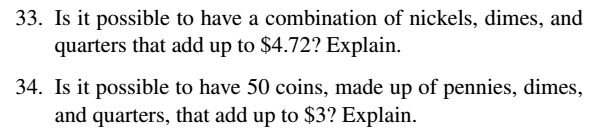
\includegraphics{HW2Prob1}
\centering
\end{figure}
\begin{large}
\section*{Problem 33}
I'm going to remove the \$ and just have a nickle = 5, dime = 10, and quarter = 25. \newline
This question asks if $5x + 10y + 25z = 472$ is solvable when (x,y,z) $\epsilon$ $\mathbf{Z}^+$
\newline\newline 
\textbf{Solution}: Because 5,10,25 are all divisible by 5, any combination of their sums is also divisible by 5. 472 on the other hand is not divisible by 5, so there is no way that a combination of 5,10,25 could combine to make 472. 
\newline \newline 
Additionally, 472's prime factors are 2,2,2,59. None of which multiply to equal 5, 10, or 25.

\section*{Problem 34}
Similar to problem 33, this question asks if the following equation is solvable

\begin{align}
\cases
{
x + 10y + 25z &= 300\\
x + y + z &= 50\\
(x,y,z) &\epsilon \mathbf{Z}^+
}
\end{align}


\textbf{Solution}: If you subtract the 2nd equation from the 1st, you get 9y + 24z = 250. \newline
This can be factored into $3(3y+8z)=250$. $3y+8z$ is some integer (m) because the product and addition of integers is another integer. So you end up with $3*(m) = 250$. 250 is not evenly divisible by 3, therefore no integer value is a solution to the problem. 

% PROBLEM 2 --------------------------------------------------------
\problem{2}
\collab{none}
\clearpage
\header

\section*{Section 4.4, Problem 15}

\begin{figure}[h]
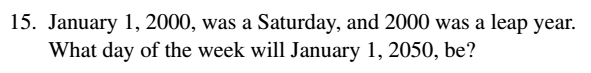
\includegraphics{HW2Prob2}
\centering
\end{figure}

\begin{itemize}
 \item A leap year happens every 4 years and there is 1 extra day on a leap year.
 \item Every non-leap year causes a shift of 1 day forward in the week compared to the previous year. 
\item A leap year causes a shift of 2 days in the week compared to the previous year.
\end{itemize}
\textbf{Solution}: Between Jan 1, 2000 and Jan 1, 2050, there will be 13 leap days. (50/4) = 12 (leap years between 2000 and 2050 (noninclusive)) + 1 (for year 2000's leap day that hadn't occurred yet). \newline \newline
So the equation can be written as: Days Offset = 2$*$Leap years $+$ non-leap years. 
\newline = $2*13 + 37$ 
\newline = 63 days offset
\newline (Days Offset) mod (7) = the shift forward in the specific day of the week, but here it results in 0, meaning that Jan 1, 2050 will be the same day of the week as Jan 1, 2000 which was a \textbf{Saturday}.

%PROBLEM 3 ----------------------------------------------------------
\problem{3}
\collab{none}
\clearpage
\header

\section*{Section 4.4, Problem 35}

\begin{figure}[h]
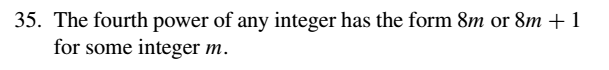
\includegraphics{HW2Prob3}
\centering
\end{figure}



\begin{itemize}
    \item This problem asks to prove that $n^4 = 8m$ or $n^4 = 8m + 1$. \newline
    \item I chose to split the problem into 2 cases: 
    \begin{enumerate}
        \item n is even
        \item n is odd
    \end{enumerate}
\end{itemize}
\textbf{Solution}:\newline 
\textbf{If n is even:} \newline 
Let n be some even integer such that n = 2k. \newline
$n^4$ where (n = 2k) results in $n^4 = 16k^4$. $k^4$ is just some integer
\newline
$(16*$ some-int) mod (8) = 0 because 16 is evenly divisible by 8. 
\newline This matches the form $n^4 = 8m$ \newline \newline
\textbf{If n is odd:} \newline
Let n be some odd integer such that n = 2k + 1 \newline
$n^4$ where (n = 2k + 1) results in \newline $16k^4 + 32k^3 + 24k^2 + 8k + 1$ \newline
$= 8(2k^4 + 4k^3 + 3k^2 + k) + 1$ \newline
$(2k^4 + 4k^3 + 3k^2 + k)$ is just some integer so it can be rewritten as: \newline
$(8*$ some-int + 1) mod (8) = 1 because the $8*x$ portion will equal 0 and (1)mod(8) = 1
\newline This matches the form $n^4 = 8m + 1$ \newline
\newline \textbf{Conclusion}: If n is even: $n^4 = 8m$, if n is odd: $n^4 = 8m + 1$

%PROBLEM 4 -----------------------------------------------------------
\problem{4}
\collab{none}
\clearpage
\header

\section*{Section 9.2, Problem 10}

\begin{figure}[h]
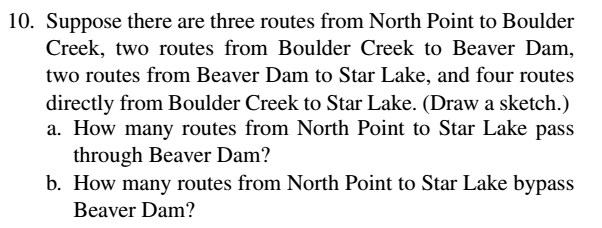
\includegraphics[scale = 0.9]{HW2Prob4}
\centering
\end{figure}

\begin{figure}[h]
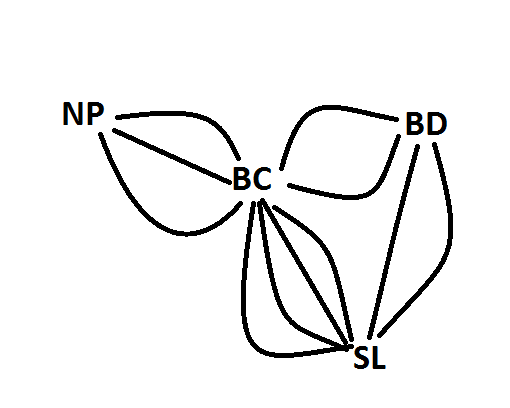
\includegraphics[scale = 0.7]{HW2Prob4-a}
\caption{A Mediocre drawing of the paths between locations}
\centering
\end{figure}

\textbf{Solution}: I will be abbreviating the names of the locations (as I did in the drawing).
\begin{enumerate}[(a)]
    \item There are 3 routes from NP $\rightarrow$ BC, 
        \newline There are 2 routes from BC $\rightarrow$ BD,
        \newline And there are 2 routes from BD $\rightarrow$ SL.
        \newline \textbf{Therefore,} there are a total of $3*2*2 = 12$ ways to get from NP $\rightarrow$ SL through BD. (multiplication rule).
        
    \item There are 3 routes from NP $\rightarrow$ BC 
        \newline And 4 routes from BC $\rightarrow$ SL.
        \newline \textbf{Therefore,} there are 12 routes that bypass BD.
\end{enumerate}

%PROBLEM 5 ------------------------------------------------------------
\problem{5}
\collab{none}
\clearpage
\header

\section*{Section 9.6, Problem 7}

\begin{figure}[h]
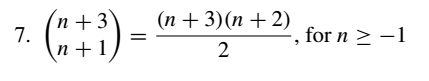
\includegraphics[scale = 1]{HW2Prob5}
\centering
\end{figure}

This problem asks to either justify the equation by either deriving from formulas or by direct computation from Theorem 9.5.1. 

\begin{figure}[h]
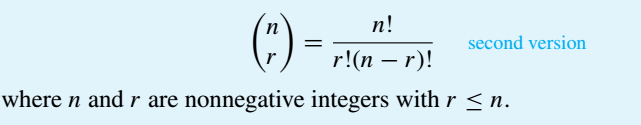
\includegraphics[scale = 1]{HW2Prob5-a}
\centering
\end{figure}

\textbf{Solution}:
\begingroup
\addtolength{\jot}{1em}
\begin{align*}
    \binom{n+3}{n+1} &= \frac{(n+3)!}{(n+1)!((n+3)-(n-1))!} \\
                     &= \frac{(n+3)!}{(n+1)!(2)!} \\
                     &= \frac{(n+3)!}{(n+1)!(2)} * \frac{(n+2)(n+3)}{(n+2)(n+3)} \\
                     &= \frac{(n+3)!(n+2)(n+3)}{(n+1)!(n+2)(n+3)(2)} \\
                     &= \frac{(n+3)!(n+2)(n+3)}{(n+3)!(2)} \\
                     &= \frac{(n+2)(n+3)}{2}
\end{align*}
\endgroup

%Problem 6 -----------------------------------------------------------------------
\problem{6}
\collab{none}
\clearpage
\header

\section*{Section 9.6, Problem 32}

\begin{figure}[h]
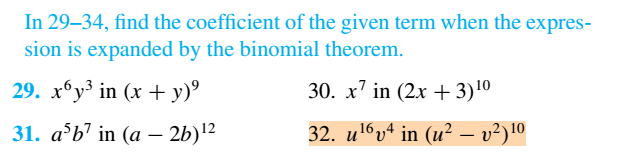
\includegraphics[scale = 1]{HW2Prob6}
\centering
\end{figure}

\begingroup
\addtolength{\jot}{1em}
\begin{align*}
    (a+b)^n &= \sum_{k=0}^{n} \binom{n}{k} a^{n-k}b^{k} \\
    (u^2-v^2)^{10} &= \sum_{k=0}^{10} \binom{10}{k} (u^2)^{10-k}(-v^2)^{k} \\
                   &= \binom{10}{0} (u^2)^{10}(-v^2)^{0} + \binom{10}{1} (u^2)^{9}(-v^2)^{1} 
                   + \boxed{\binom{10}{2} (u^2)^{8}(-v^2)^{2}} \\
                   &= \binom{10}{2} (u^{16})(v^4) \\
                   \text{coefficient} &= \binom{10}{2}
                   = \frac{10!}{(2!)(8!)}
                   = \frac{10*9}{2} = 45
\end{align*}
\endgroup

%Problem 7 ------------------------------------------------------------------------------------
\problem{7}
\collab{none}
\clearpage
\header

\begin{figure}[h]
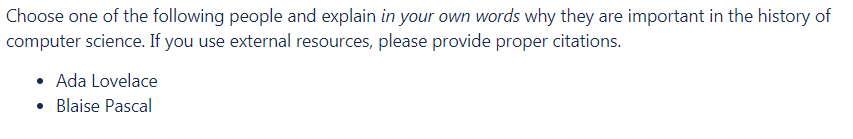
\includegraphics[scale = 1]{HW2Prob7}
\centering
\end{figure}

Ada Lovelace helped work on Charles Babbage's Analytical Engine that was designed to compute logarithms, trigonometric functions, and approximate polynomials. What makes her so important is that she was the first to realize that "analytical engines" could solve problems beyond number crunching. If you could represent other things as numbers, you could manipulate them just the same. This idea was by no means obvious, and essentially predicted the way modern computers would function over a hundred years later. \\


Source: “Ada Lovelace,” Wikipedia, 09-Sep-2018. [Online]. Available: \url{https://en.wikipedia.org/wiki/Ada_Lovelace}. [Accessed: 12-Sep-2018].


\end{large}
\end{document}